\documentclass[]{tufte-book}

% ams
\usepackage{amssymb,amsmath}

\usepackage{ifxetex,ifluatex}
\usepackage{fixltx2e} % provides \textsubscript
\ifnum 0\ifxetex 1\fi\ifluatex 1\fi=0 % if pdftex
  \usepackage[T1]{fontenc}
  \usepackage[utf8]{inputenc}
\else % if luatex or xelatex
  \makeatletter
  \@ifpackageloaded{fontspec}{}{\usepackage{fontspec}}
  \makeatother
  \defaultfontfeatures{Ligatures=TeX,Scale=MatchLowercase}
  \makeatletter
  \@ifpackageloaded{soul}{
     \renewcommand\allcapsspacing[1]{{\addfontfeature{LetterSpace=15}#1}}
     \renewcommand\smallcapsspacing[1]{{\addfontfeature{LetterSpace=10}#1}}
   }{}
  \makeatother

\fi

% graphix
\usepackage{graphicx}
\setkeys{Gin}{width=\linewidth,totalheight=\textheight,keepaspectratio}

% booktabs
\usepackage{booktabs}

% url
\usepackage{url}

% hyperref
\usepackage{hyperref}

% units.
\usepackage{units}


\setcounter{secnumdepth}{-1}

% citations


% pandoc syntax highlighting

% longtable

% multiplecol
\usepackage{multicol}

% strikeout
\usepackage[normalem]{ulem}

% morefloats
\usepackage{morefloats}


% tightlist macro required by pandoc >= 1.14
\providecommand{\tightlist}{%
  \setlength{\itemsep}{0pt}\setlength{\parskip}{0pt}}

% title / author / date
\title{Development Research in Practice}
\author{Kristoffer Bjarkefur, Luiza Cardoso de Andrade, Benjamin Daniels, Maria
Ruth Jones}
\date{}


\begin{document}

\maketitle




\hypertarget{acknowledgments-and-notes}{%
\chapter*{Acknowledgments and notes}\label{acknowledgments-and-notes}}
\addcontentsline{toc}{chapter}{Acknowledgments and notes}

We want to thank all the people who helped us get here, especially
Arianna Legovini, for her leadership at DIME, unending support of our
work, and detailed comments on this book; and Florence Kondylis, for her
leadership in founding and growing DIME Analytics and supporting this
project from the very first. We also thank the following members of DIME
Analytics for their contributions to the ideas in this book and their
help organizing them: Roshni Khincha, Avnish Singh, Patricia Paskov,
Radhika Kaul, Mizuhiro Suzuki, Yifan Powers, and Maria Arnal Canudo.
This work has been financially supported by the United Kingdom Foreign,
Commonwealth \& Development Office (FCDO) through the DIME i2i Umbrella
Facility for Impact Evaluation at the World Bank.

Our graditude to the many people who read and offered feedback as the
book took shape: Stephanie Annijas, Maria Camila Ayala Guerrero,
Kaustubh Chahande, Thomas Escande, Aram Gassama, Steven Glover, Nausheen
Khan, Robert Norling, Michael Orevba, Caio Piza, Francesco Raffaelli,
Daniel Rogger, Ankriti Singh, Ravi Somani, and Leonardo Viotti. Although
they number far too many to name individually, we also thank all the
members of DIME and its teams across all the years for the innovative
work they have done, the lessons learned, and the team spirit that makes
our work so fruitful and rewarding.

This published version of the book has been revised repeatedly since its
internal release in June 2019, with extensive feedback from readers and
experts. We would additionally like to thank Vincenzo di Maro (Manager,
DIME3) for his support throughout this process, as well as peer
reviewers David McKenzie (Lead Economist, DECFP), Holly Krambeck
(Program Manager, DECAT), Alaka Holla (Program Manager, HEDGE), Jim Shen
(Senior Manager, Abdul Latif Jameel Poverty Action Lab), Federica di
Battista (Trialling Lead, UK FCDO), and Gabriel Vicente, Rajee
Kanagavel, and Maksim Pecherskiy from the Development Data Partnership
team.

This book is a living product that is written and maintained publicly.
The code and edit history are at:
\href{https://github.com/worldbank/dime-data-handbook}{}. You can get a
PDF copy at: \href{https://worldbank.github.com/dime-data-handbook}{}.
The website includes updated instructions for providing feedback, as
well as notes on updates to the content. Whether you work with DIME, the
World Bank, or another organization or university, we ask that you read
the contents of this book critically. We welcome feedback and
corrections to improve the book. Please visit
\href{https://worldbank.github.com/dime-data-handbook/feedback}{} to
provide feedback. You can also email us at
\href{mailto:dimeanalytics@worldbank.org}{\nolinkurl{dimeanalytics@worldbank.org}},
and we will be very thankful. We hope you enjoy \emph{Development
Research in Practice}!

\hypertarget{preface}{%
\chapter*{Preface}\label{preface}}
\addcontentsline{toc}{chapter}{Preface}

Welcome to \emph{Development Research in Practice: The DIME Analytics
Data Handbook}. This book is intended to teach all users of development
data how to handle data effectively, efficiently, and ethically. An
empirical revolution has changed the face of development research
rapidly over the last decade. Increasingly, researchers are working not
just with complex data, but with \emph{original} data: datasets
collected by the research team themselves or acquired through a unique
agreement with a project partner. Research teams must carefully document
how original data is created, handled, and analyzed. These tasks now
contribute as much weight to the quality of the evidence as the research
design and the statistical approaches do. At the same time, the scope
and scale of empirical research projects is expanding: more people are
working on the same data over longer timeframes. For that reason, the
central premise of this book is that data work is a ``social process''.
This means that the many different people on a team need to have the
same ideas about what is to be done, and when and where and by whom, so
that they can collaborate effectively on a large, long-term research
project.

Despite the growing importance of managing data work, little practical
guidance is available for practitioners. There are few guides to the
conventions, standards, and best practices that are fast becoming a
necessity for empirical research. \emph{Development Research in
Practice} aims to fill that gap. It covers the full data workflow for a
complex research project using original data. We share the lessons,
tools, and processes developed within the World Bank's Development
Impact Evaluation (DIME) department, and compile them into a single
narrative of best practices for data work. This book is not
sector-specific; it will not teach you econometrics, or how to design an
impact evaluation. There are many excellent existing resources on those
topics. Instead, it will teach you how to think about all aspects of
your research from a data perspective, how to structure research
projects to ensure data quality, and how to institute transparent and
reproducible workflows. We realize that adopting these workflows may
have significant upfront learning costs, but we are convinced that these
investments pay off quickly, as you will both save time and improve the
quality of your research going forward.

\hypertarget{how-to-read-this-book}{%
\section*{How to read this book}\label{how-to-read-this-book}}
\addcontentsline{toc}{section}{How to read this book}

This book aims to be a highly practical resource so the reader can
immediately begin to collaborate more effectively on large, long-term
research projects that use the methods and tools discussed. This
introduction outlines the basic philosophies that motivate this book and
our approach to research data. We want all readers to understand at the
outset our mindset that research data work is primarily about
communicating effectively within a team and that standardization and
simplification of data tasks is a major enabler of effective
collaboration. The main chapters of this book will walk you through the
data workflow at each stage of an empirical research project, from
design to publication. The figure in this introduction visualizes the
data workflow. Chapters 1 and 2 contextualize the workflow, and set the
stage for the hands-on data tasks which are described in detail in
Chapters 3 to 7.

\textbf{Chapter 1} This book aims to be a highly practical resource so
the reader can immediately begin to collaborate more effectively on
large, long-term research projects that use the methods and tools
discussed. This introduction outlines the basic philosophies that
motivate this book and our approach to research data. We want all
readers to understand at the outset our mindset that research data work
is primarily about communicating effectively within a team and that
standardization and simplification of data tasks is a major enabler of
effective collaboration. The main chapters of this book will walk you
through the data workflow at each stage of an empirical research
project, from design to publication. The figure in this introduction
visualizes the data workflow. Chapters 1 and 2 contextualize the
workflow, and set the stage for the hands-on data tasks which are
described in detail in Chapters 3 to 7.

\textbf{Chapter 2} teaches you to structure your data work for
collaborative research, while ensuring the privacy and security of
research participants. It discusses the importance of planning data work
and associated tools in advance, long before any data is acquired. It
also describes ethical concerns common to development data, common
pitfalls in legal and practical management of data, and how to respect
the rights of research participants at all stages of data work

\textbf{Chapter 3} turns to the measurement framework, and how to
translate research design to a data work plan. It details DIME's data
map template, a set of tools to communicate the project's data
requirements both across the team and across time. It also discusses how
to implement random sampling and random assignment in a reproducible and
credible manner.

\textbf{Chapter 4} covers data acquisition. It starts with the legal and
institutional frameworks for data ownership and licensing, to ensure
that you are aware of the rights and responsibilities of using data
collected by the research team or by others. It provides a deep dive on
collecting high-quality primary electronic survey data, including
developing and deploying survey instruments. Finally, it discusses
secure data handling during transfer, sharing, and storage, which is
essential in protecting the privacy of respondents in any data.

\textbf{Chapter 5} describes data processing tasks. It details how to
construct ``tidy'' data at the appropriate units of analysis, how to
ensure uniquely identified datasets, and how to routinely incorporate
data quality checks into the workflow. It also provides guidance on
de-identification and cleaning of personally-identified data, focusing
on how to understand and structure data so that it is ready for
indicator construction and analytical work.

\textbf{Chapter 6} discusses data analysis tasks. It begins with data
construction, or the creation of new variables from the raw data
acquired or collected in the field. It introduces core principles for
writing analytical code and creating, exporting, and storing research
outputs such as figures and tables reproducibly using dynamic documents.

\textbf{Chapter 7} outlines the publication of research outputs,
including manuscripts, code, and data. This chapter discusses how to
effectively collaborate on technical writing using dynamic documents. It
also covers how and why to publish datasets in an accessible, citable,
and safe fashion. Finally, it provides guidelines for preparing
functional and informative reproducibility packages that contain all the
code, data, and meta-information needed for others to evaluate and
reproduce your work.

Each chapter starts with a box which provides a summary of the most
important points, takeaways for different types of readers, and a list
of key tools and resources for implementing the recommended practices.
After reading each chapter, you should understand what tasks will be
performed at every stage of the workflow, and how to implement them
according to best practices. You should also understand how the various
stages of the workflow tie together, and what inputs and outputs are
required and produced from each. The references and links contained in
each chapter will lead you to detailed descriptions of individual ideas,
tools, and processes to refer to when you need to implement the tasks
yourself.

\BeginKnitrBlock{example}

\hypertarget{demand-for-safe-spaces-case-study}{%
\chapter{Demand for Safe Spaces Case
Study}\label{demand-for-safe-spaces-case-study}}

Throughout this Handbook, we will refer to a completed DIME project,
\emph{Demand for Safe Spaces: Avoiding Harassment and Stigma}, to
provide a case study of the empirical research tasks described in this
book. You will find boxes in each chapter with examples of how the
practices and workflows described in that chapter were applied in this
real-life example. All the code examples and diagrams referenced in the
case study can be accessed directly through this book's GitHub
repository. We have made minor adaptations to the original study
materials presented for function and clarity. All original materials can
be found in the project's reproducibility package.

\textbf{The \emph{Demand for Safe Spaces} study is summarized in its
abstract as follows.} What are the costs to women of harassment on
public transit? This study randomizes the price of a women-reserved
``safe space'' in Rio de Janeiro and crowdsource information on 22,000
rides. Women in the public space experience harassment once a week. A
fifth of riders are willing to forgo 20 percent of the fare to ride in
the ``safe space''. Randomly assigning riders to the ``safe space''
reduces physical harassment by 50 percent, implying a cost of \$1.45 per
incident. Implicit Association Tests show that women face a stigma for
riding in the public space that may outweigh the benefits of the safe
space.

The Demand for Safe Spaces study used novel original data from three
sources. It collected information on 22,000 metro rides from a
crowdsourcing app (referred to as \emph{crowdsourced ride data} in the
case study examples), a survey of randomly-sampled commuters on the
platform (referred to as the \emph{platform survey}), and data from an
\emph{implicit association test}. The research team first elicited
revealed preferences for the women-reserved cars, and then randomly
assigned riders across the reserved and non-reserved cars to measure
differences in the incidence of harassment. The use of a customized app
allowed the researchers to assign data collection tasks and vary
assigned ride spaces (women-reserved car vs public cars) and associated
payout across rides. In addition, the team administered social norm
surveys and implicit associations tests on a random sample of men and
women commuters to document a potential side effect of reserved spaces:
stigma against women who choose to ride in the public space.

For the purposes of the Handbook, we focus on the protocols, methods,
and data used in the \emph{Demand for Safe Spaces study}, rather than
the results. To learn more about the findings from this study, and more
details on how it was conducted, we encourage readers to download the
working paper. The material from all the examples in the book and be
found at
\url{https://github.com/worldbank/dime-data-handbook/tree/master/examples}.

\begin{itemize}
\item
  The Demand for Safe Spaces study repository can be accessed at
  \url{https://github.com/worldbank/rio-safe-space}.
\item
  The working paper \emph{Demand for Safe Spaces: Avoiding Harassment
  and Stigma} is available at
  \url{https://openknowledge.worldbank.org/handle/10986/33853}.
\end{itemize}

\EndKnitrBlock{example}

\hypertarget{the-dime-wiki-a-complementary-resource}{%
\section*{The DIME Wiki: A complementary
resource}\label{the-dime-wiki-a-complementary-resource}}
\addcontentsline{toc}{section}{The DIME Wiki: A complementary resource}

Throughout the book, you will find many references to the DIME Wiki. The
DIME Wiki is a free online collection of impact evaluation resources and
best practices. This handbook and the DIME Wiki are meant to go
hand-in-hand: the handbook provides the narrative structure and
workflow, and the Wiki dives into specific implementation details,
offers detailed code examples, and provides a more exhaustive set of
references for each topic. Importantly, the DIME Wiki is a living
resource that is continuously updated and improved, by the authors of
this book and external contributors. We welcome all readers to
\href{https://dimewiki.worldbank.org/New_Users}{register as Wiki users}
and contribute directly.

\begin{figure}
\centering
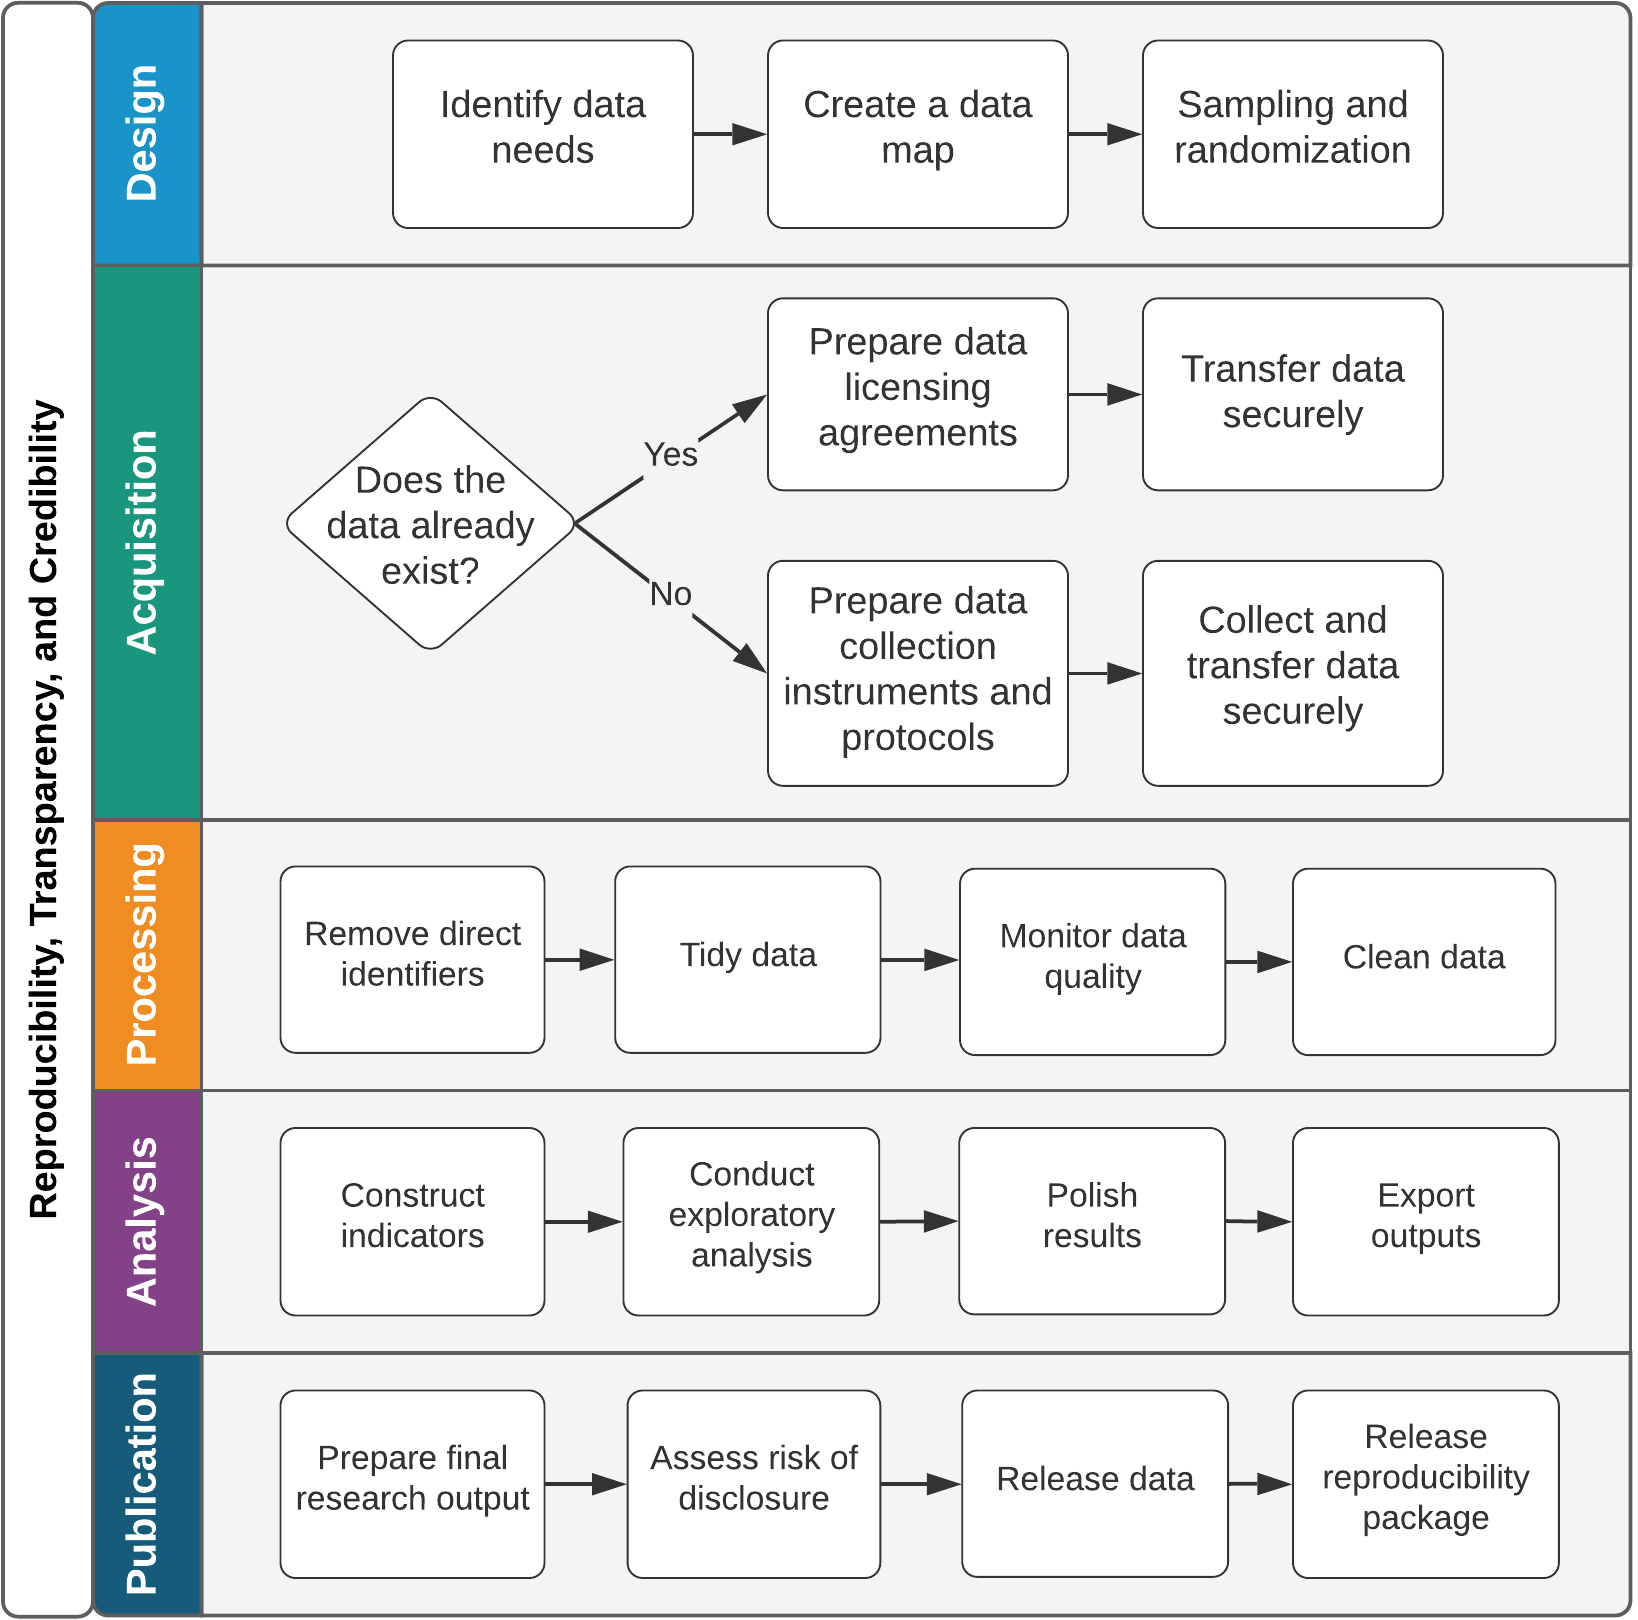
\includegraphics{../diagrams/Introduction.png}
\caption{Overview of development research data work tasks}
\end{figure}

\hypertarget{standardizing-data-work}{%
\section*{Standardizing data work}\label{standardizing-data-work}}
\addcontentsline{toc}{section}{Standardizing data work}

In the past, data work was often treated as a ``black box'' in research.
A published manuscript might exhaustively detail research designs,
estimation strategies, and theoretical frameworks, but typically
reserved very little space for detailed descriptions of how data was
actually collected and handled. It is almost impossible to assess the
quality of the data in such a paper, and whether the results could be
reproduced. In the past decade, this has started to change,\footnote{\citet{swanson2020research}}
in part due to increasing requirements by publishers and funders to
release code and data.

Data handling and documentation is a key skill for researchers and
research staff. Standard processes and documentation practices are
important throughout the research process to accurately convey and
implement the intended research design, and to minimizes security risks:
better protocols and processes lower the probability of data leakages,
security breaches, and loss of personal information. When data work is
done in an ad-hoc manner, it is very difficult for others to understand
what is being done -- a reader has to simply trust that the researchers
did these things right. Most importantly, if any part of the data
pipeline breaks down, research results become unreliable and cannot be
faithfully interpreted as being an accurate picture of the intended
research design. Because we almost never have ``laboratory'' settings in
this type of research, such a failure has a very high cost: we will have
wasted the investments that were made into knowledge generation, and the
research opportunity itself, where we intended to conduct the study.
Accurate and reproducible data management and analysis is essential to
the success and credibility of modern research. Standardizing and
documenting data handling processes is essential to be able to evaluate
and understand the data work alongside any final research outputs. An
important component of this is process standardization. Process
standardization means that there is little ambiguity about how something
ought to be done, and therefore the tools to do it can be set in
advance. Standard processes help other people understand your work, and
they also make your work easier to document. Process standardization and
documentation should allow readers of your code to: (1) quickly
understand what a particular process or output is supposed to be doing;
(2) evaluate whether or not it does that thing correctly; and (3) modify
it either to test alternative hypotheses or to adapt into their own
work. This book will discuss specific standards recommended by DIME
Analytics, but we are more interested in convincing the reader to
discuss the adoption of a standard within research teams than to
necessarily use the particular standards that we recommend.

\hypertarget{conducting-reproducible-transparent-and-credible-research}{%
\chapter{Conducting reproducible, transparent, and credible
research}\label{conducting-reproducible-transparent-and-credible-research}}

Policy decisions are made every day using the results of development
research, and these have wide-reaching effects on the lives of millions.
As the emphasis on evidence-based policy grows, so too does the scrutiny
under which research methods and results are placed. Three major
components make up this scrutiny: credibility, transparency, and
reproducibility. These three components contribute to one simple idea:
research should be high quality and well-documented. Research consumers,
including the policy makers who will use the evidence to make decisions,
should be able to easily examine and recreate such evidence. In this
framework, it is useful to think of research as a public service that
requires researchers as a group to be accountable for their methods.
This means acting to collectively protect the credibility of development
research by following modern practices for research planning and
documentation. Across the social sciences, the open science movement has
been fueled by concerns about the proliferation of low-quality research
practices, data and code that are inaccessible to the public, analytical
errors in major research papers, and in some cases even outright fraud.
While the development research community has not yet experienced major
scandals, it has become clear that there are necessary improvements to
make in the way that code and data are handled as part of research.
Moreover, having common standards and practices for creating and sharing
materials, code, and data with others will improve the value of the work
we do.

In this chapter, we outline principles and practices that help to ensure
research consumers can be confident in the conclusions reached. We
discuss each of the three components -- credibility, transparency, and
reproducibility -- in turn. The first section covers research
credibility. It presents three popular methods to commit to particular
research questions or methods, and avoid potential criticisms of
cherry-picking results: registration, pre-analysis plans, and registered
reports. The second section discusses how to apply principles of
transparency to all research processes, which allows research teams to
be more efficient, and research consumers to fully understand and
evaluate research quality. The final section provides guidance on how to
make your research fully reproducible, and explains why publishing
replication materials is an important research contribution in its own
right.

\hypertarget{developing-a-credible-research-project}{%
\section*{Developing a credible research
project}\label{developing-a-credible-research-project}}
\addcontentsline{toc}{section}{Developing a credible research project}

The evidentiary value of research is traditionally a function of design
choices,\footnote{\cite{@angrist2010credibility},\cite{@ioannidis2005most}}
such as powered through sampling and randomization, and robustness to
alternative specifications and definitions. One frequent target for
critics of such research\footnote{\cite{@ioannidis2017power}} is the
fact that most researchers have a lot of leeway in selecting their
projects, results, or outcomes \emph{after} already having had the
experience of implementing a project or collecting data in the field,
which increases the likelihood of finding ``false positive'' results
that are not true outside carefully-selected data.\footnote{\cite{@simmons2011false}}
Credible research design methods are key to maintaining credibility in
these choices and avoiding serious errors. This is especially relevant
for research that relies on original data sources, from innovative big
data sources to unique surveys. Development researchers should take
these concerns seriously. Such flexibility can be a significant issue
for the quality of evidence overall, particularly if researchers believe
that certain types of results are substantially better for their careers
or their publication chances.

This section presents three popular methods for researchers to commit to
particular research questions or methods, and to avoid potential
criticisms of cherry-picking results for publication: registration,
pre-analysis plans, and registered
reports.\index{registration}\index{pre-analysis plans}\index{registered reports}
Each of these methods involves documenting specific research design
components, ideally before carrying out the analytical component or
extensively exploring the data. Study registration provides formal
notice that a study is being attempted and creates a hub for materials
and updates about the study results. Pre-analysis plans are a more
formal commitment to use specific methods on particular questions.
Writing and releasing a pre-analysis plan in advance of working with
data is used to protect the credibility of approaches that have a high
likelihood of producing false results.\footnote{\cite{@wicherts2016degrees}}
Finally, registered reports allow researchers to approach research
planning itself as a process at the level of a full peer review.
Registered reports enable close scrutiny of a research design, a
feedback and improvement process, and a commitment from a publisher to
publish the study based on the credibility of the design, rather than
the specific results.

\hypertarget{registering-research-studies}{%
\subsection*{Registering research
studies}\label{registering-research-studies}}
\addcontentsline{toc}{subsection}{Registering research studies}

Registration of research studies is an increasingly common practice, and
more journals are beginning to require the registration of studies they
publish.\footnote{\cite{@vilhuber2020report}} Study registration
intended to ensure that a complete record of research inquiry is easily
available.\footnote{\href{https://dimewiki.worldbank.org/Study_Registration}{}}
Registering research studies ensures that future scholars can quickly
find out what work has been carried out on a given question, even if
some or all of the work done never results in formal publication.
Registration of studies is increasingly required by publishers and can
be done before, during, or after the study with essential information
about the study purpose. Some currently popular registries are operated
by the \href{https://www.socialscienceregistry.org}{\textbf{AEA}},
\href{https://ridie.3ieimpact.org}{\textbf{3ie}},
\href{https://egap.org/content/registration}{\textbf{eGAP}}, and
\href{https://osf.io/registries}{\textbf{OSF}}. They all have different
target audiences and features, so select one that is appropriate to your
work. \index{pre-registration}

Pre-registering studies before they begin is an extension of this
principle.\footnote{\cite{@nosek2018preregistration}} Registration of a
study before it goes to implementation or data acquisition, particularly
when specific hypotheses are included in the registration, provides a
simple and low-effort way for researchers to conclusively demonstrate
that a particular line of inquiry was not generated by the process of
data collection or analysis itself.\footnote{\href{https://dimewiki.worldbank.org/Pre-Registration}{}}\index{pre-registration}
Pre-registrations need not provide exhaustive details about how a
particular hypothesis will be approached; only that it will be. This can
be highly valuable for the credibility of the research and requires only
minor time investment or administrative effort. For this reason, the
DIME team requires pre-registration of all studies in a public database
with at least some primary hypotheses prespecified, prior to providing
funding for impact evaluation research.

\hypertarget{writing-pre-analysis-plans}{%
\subsection*{Writing pre-analysis
plans}\label{writing-pre-analysis-plans}}
\addcontentsline{toc}{subsection}{Writing pre-analysis plans}

If a research team has a large amount of flexibility to define how they
approach a particular hypothesis, study registration may not be
sufficient to avoid the criticism of ``hypothesizing after the results
are known'', or HARKing.\footnote{\cite{@kerr1998harking}} Examples of
such flexibility include a broad range of concrete measures that could
be argued to measure to an abstract concept; future choices about sample
inclusion or exclusion; or decisions about how to construct derived
indicators. When the researcher is collecting a large amount of
information and has leverage over even a moderate number of these
options, it is almost guaranteed that they can come up with any result
they like.\footnote{\cite{@gelman2013garden}}

\href{https://dimewiki.worldbank.org/Pre-Analysis_Plan}{Pre-analysis
plans (PAPs)}\index{pre-analysis plan} can be used to assuage these
concerns by specifying some set of analyses the researchers intend to
conduct. The pre-analysis plan should be written up in detail for areas
that are known to provide a large amount of leeway for researchers to
make later decisions, particularly for things like interaction effects
or subgroup analysis.\footnote{See \cite{@cusolito2018can} for an
  example.} Pre-analysis plans shoud not, however, be viewed as binding
the researcher's hands.\footnote{\cite{@olken2015promises}} Depending on
what is known about the study at the time of writing, pre-analysis plans
can vary widely in the amount of detail they should include.\footnote{\href{https://blogs.worldbank.org/impactevaluations/pre-analysis-plans-and-registered-reports-what-new-opinion-piece-does-and-doesnt}{}}
The core function of a PAP is to carefully and explicitly describe one
or more specific data-driven inquiries, as specific formulations are
often very hard to justify in retrospect with data or projects that
potentially provide many avenues to approach a single theoretical
question.\footnote{See \cite{@bedoya2019no} for an example.} Anything
outside the original plan is just as interesting and valuable as it
would have been if the the plan was never published; but having
pre-committed to the details of a particular inquiry makes its results
immune to a wide range of criticisms of specification searching or
multiple testing.\footnote{\cite{@duflo2020praise}}

\hypertarget{publishing-registered-reports}{%
\subsection*{Publishing registered
reports}\label{publishing-registered-reports}}
\addcontentsline{toc}{subsection}{Publishing registered reports}

\href{https://dimewiki.worldbank.org/Registered_Reports}{\textbf{Registered
reports}}\index{registered reports} take the process of pre-specifying a
complex research design to the level of a formal publication. In a
registered report, a journal or other publisher will peer review and
conditionally accept a specific study for publication, typically then
guaranteeing the acceptance of a later publication that carries out the
analysis described in the registered report. While far stricter and more
complex to carry out than ordinary study registration or pre-analysis
planning, the registered report has the added benefit of peer review and
expert feedback on the design and structure of the proposed
study.\footnote{\href{https://blogs.worldbank.org/impactevaluations/registered-reports-piloting-pre-results-review-process-journal-development-economics}{}}

This process is in part meant to combat the ``file-drawer
problem''\footnote{\cite{@simonsohn2014p}}\index{file-drawer problem}
and ensure that researchers are transparent in the sense that all
promised results obtained from registered-report studies are actually
published. This approach has the advantage of pre-specifying in great
detail a complete research and analytical design, and securing a
commitment for publication regardless of the outcome. This may be of
special interest for researchers studying events or programs where
either there is a substantial risk that they would either not be able to
publish a null or negative result,\footnote{See
  \cite{@coville2019nollywood} for an example.}\index{null result} or
where they may wish to avoid any pressure toward finding a particular
result, for example when the program or event is the subject of
substantial social or political pressures. As with pre-registration and
pre-analysis, nothing in a registered report should be understood to
prevent a researcher from pursuing additional avenures of inquiry once
the study is complete, either in the same or separate research outputs.

\hypertarget{conducting-research-transparently}{%
\section*{Conducting research
transparently}\label{conducting-research-transparently}}
\addcontentsline{toc}{section}{Conducting research transparently}

Transparent research exposes not only the code, but all research
processes involved in developing the analytical approach. This means
that readers are able to judge for themselves whether the research was
done well and the decision-making process was sound. If the research is
well-structured, and all of the relevant documentation\footnote{\href{https://dimewiki.worldbank.org/Research_Documentation}{}}\index{research documentation}
is shared, it is easy for the reader to understand the analysis fully.
Researchers that expect process transparency also have an incentive to
make better decisions, be skeptical and thorough about their
assumptions, and save themselves time, because transparent research
methods are labor-saving over the complete course of a project.

Clearly documenting research work is necessary to allow others to
evaluate exactly what data was acquired and how it was used to obtain a
particular result. Many development research projects are purpose-built
to address specific questions, and often use unique data, novel methods,
or small samples. These approaches can yield new insights into essential
academic questions, but need to be transparently documented so they can
be reviewed or replicated by others in the future.\footnote{\cite{@duvendack2017meant}}
Unlike disciplines where data is more standardized or where research is
more oriented around secondary data, the exact data used in a
development project has often not been observed by anyone else in the
past and may not be able to be re-collected by others in the future.
Regardless of the novelty of study data, transparent documentation
methods help ensure that data was collected and handled appropriately
and that studies and interventions were implemented correctly. As with
study registrations, project and data documentation should be released
on external \textbf{archival repositories}\footnote{\textbf{Archival
  repository:}A third-party service for information storage that
  guarantees the permanent availability of current and prior versions of
  materials.}\index{archival repository} so they can always be accessed
and verified.

\hypertarget{documenting-data-acquisition-and-analysis}{%
\subsection*{Documenting data acquisition and
analysis}\label{documenting-data-acquisition-and-analysis}}
\addcontentsline{toc}{subsection}{Documenting data acquisition and
analysis}

Documenting a project in detail greatly increases transparency. Many
disciplines have a tradition of keeping a ``lab notebook'', and adapting
and expanding this process to create a lab-style workflow in the
development field is a critical step towards more transparent practices.
This means explicitly noting decisions as they are made, and explaining
the process behind the decision-making. Careful documentation will also
save the research team a lot of time during a project, as it prevents
you from having the same discussion twice (or more!), since you have a
record of why something was done in a particular way. There are a number
of available tools that will contribute to producing
documentation,\index{project documentation} but project documentation
should always be an active and ongoing process, not a one-time
requirement or retrospective task. New decisions are always being made
as the plan begins contact with reality, and there is nothing wrong with
sensible adaptation so long as it is recorded and disclosed.

Email, however, is \emph{not} a documentation service, because
communications are rarely well-ordered,\index{email} can be easily
deleted, and are not available for future team members. There are
various software solutions for building proper documentation over time.
Some work better for field records such as implementation decisions,
research design, and survey development; others work better for
recording data work and code development. The
\href{https://osf.io}{\textbf{Open Science Framework}} provides one such
solution,\index{Open Science Framework} with integrated file storage,
version histories, and collaborative wiki pages.
\href{https://github.com}{\textbf{GitHub}} provides a transparent
documentation system through commit messages, issues, \texttt{README}
files, and pull requests,\^{}{[}
\href{https://dimewiki.worldbank.org/Getting_started_with_GitHub}{}\index{task management}\index{GitHub}\index{README}
in addition to version histories and wiki pages.\index{version control}
Such services offer multiple different ways to record the decision
process leading to changes and additions, track and register
discussions, and manage tasks. These are flexible tools that can be
adapted to different team and project dynamics. Services that log your
research process can show things like modifications made in response to
referee comments, by having tagged version histories at each major
revision. They also allow you to use issue trackers to document the
research paths and questions you may have tried to answer as a resource
to others who have similar questions. Each project has specific
requirements for data, code, and documentation management, and the exact
transparency tools to use will depend on the team's needs, but they
should be agreed upon prior to project launch. This way, you can start
building a project's documentation as soon as you start making
decisions.

\hypertarget{cataloging-and-archiving-data}{%
\subsection*{Cataloging and archiving
data}\label{cataloging-and-archiving-data}}
\addcontentsline{toc}{subsection}{Cataloging and archiving data}

Data and data collection methods should be fully cataloged, archived,
and documented, whether you are collecting data yourself or receiving it
from an outside partner. In some cases this is as simple as uploading a
survey instrument or an index of datasets and a codebook to an
archive.\index{codebook} In other cases this will be more complex.
Proper documentation of data collection will often require a detailed
description of the overall sampling procedure.\footnote{See
  \cite{@yishay2016gender} for an example.} For example, settings with
many overlapping strata, treatment arms, excluded observations, or
resampling protocols might require extensive additional field work
documentation. This documentation should be continuously updated and
kept with the other study materials; it is often necessary to collate
these materials for an appendix for publication in any case.

When data is recieved from partners or collected in the field, the
\textbf{original data} (including corrections)\footnote{\textbf{Original
  data:} A new dataset, as obtained and corrected, that becomes the
  functional basis for research work.}\index{original data} should be
immediately placed in a secure permanent storage system. Before
analytical work begins, you should create a ``for-publication'' copy of
the original dataset by removing potentially identifying
information.\index{de-identification} This will become the raw data, and
must be placed in an archival repository where it can be
cited.\footnote{\cite{@vilhuber2020report}}\index{data publication} This
can initially be done under embargo or with limited release, in order to
protect your data and future work. This type of data depositing or
archiving precedes publishing or releasing any data: data at this stage
may still need to be embargoed or have other, potentially permanent,
access restrictions, so you can instruct the archive to formally release
the data later.

Some project funders provide specific repositories in which they require
the deposit of data they funded,\footnote{For example,
  \href{https://data.usaid.gov}{}} and you should take advantage of
these when possible. If this is not provided, you must be aware of
privacy issues with directly identifying data and questions of data
ownership before uploading raw data to any third-party server, whether
public or not;\index{data ownership} this is a legal question for your
home organization. Regardless of these consideration, all data
repositories, such as DIME's standard, the
\href{https://microdata.worldbank.org}{World Bank Microdata Library} and
the \href{https:/datacatalog.worldbank.org}{World Bank Data Catalog},
should create a record of the data's existence and provide instructions
on how access might be obtained by another researcher. For more on the
steps required to prepare and publish a de-identified dataset, you can
refer to Chapter 6 and Chapter 7 of this book. Data publication should
create a data citation and a \textbf{digital object identifier
(DOI)},\footnote{\textbf{Digital object identifier (DOI):} A permanent
  reference for electronic information that persistently updates to a
  new URL or other locations if the information is relocated.}\index{digital object identifier (DOI)}\index{data citation}
or some other persistent index that you can use in your future work to
unambiguously indicate the location of your data. This data publication
should also include the methodological documentation as well as complete
human-readable codebooks for all the variables there.

\hypertarget{analyzing-data-reproducibly}{%
\section*{Analyzing data
reproducibly}\label{analyzing-data-reproducibly}}
\addcontentsline{toc}{section}{Analyzing data reproducibly}

Reproducible research makes it easy for others to apply your techniques
to new data or to implement a similar research design in a different
context. Development research is rapidly moving in the direction of
requiring adherence to specific reproducibility guidelines.\footnote{\cite{@christensen2018transparency}}
Major publishers and funders, most notably the American Economic
Association, have taken steps to require that code and data are
accurately reported, cited, and preserved as research outputs that can
be accessed and verified by others. Making research reproducible in this
way is a public good.\footnote{\href{https://dimewiki.worldbank.org/Reproducible_Research}{}}
It enables other researchers to re-use code and processes to do their
own work more easily and effectively in the future. Regardless of what
is formally required, your code should be written neatly with clear
instructions. It should be easy to read and understand. The
corresponding analysis data should also be made accessible to the
greatest legal and ethical extent that it can be.\footnote{\href{https://dimewiki.worldbank.org/Publishing_Data}{}}

Common research standards from journals and funders feature both
regulation and and verification policies.\footnote{\cite{@stodden2013toward}}
Regulation policies require that authors provide reproducibility
packages before publication which are then reviewed by the journal for
completeness. Verification policies require that authors make certain
materials available to the public, but their completeness is not a
precondition for publication. Other journals have adopted guidance that
offer checklists for reporting on whether and how various practices were
implemented, without specifically requiring any.\footnote{\cite{@nosek2015promoting}}
If you are personally or professionally motivated by citations,
producing these kinds of resources can lead to that as well.

\hypertarget{preparing-a-reproducibility-package}{%
\subsection*{Preparing a reproducibility
package}\label{preparing-a-reproducibility-package}}
\addcontentsline{toc}{subsection}{Preparing a reproducibility package}

At DIME, all research outputs are required to satisfy
\textbf{computational reproducibility},\footnote{\textbf{Computational
  reproducibility:} The ability of another individual to reuse the same
  code and data and obtain the exact same results as yours.}\index{computational reproducibility}
which is an increasingly common requirement for publication.\footnote{\href{https://dimewiki.worldbank.org/Reproducible_Research}{}}
Before releasing a working paper, the research team submits a
\textbf{reproducibility package} with de-identified
data,\index{reproducibility package} and DIME Analytics verifies that
the package produces exactly the same results that appear in the
paper.\footnote{\href{https://blogs.worldbank.org/impactevaluations/what-development-economists-talk-about-when-they-talk-about-reproducibility}{}}
The team also comments on whether the package includes sufficient
documentation. The Analytics team organizes frequent peer code review
for works in progress,\index{code review} and our general recommendation
is to ensure that projects are \emph{always} externally reproducible
instead of waiting until the final stages to prepare this material. Once
the computational reproducibility check is complete, the team receives a
completed reproducibility certificate that also lists any publicly
available materials to accompany the package, for use as an appendix to
the publication. The team also organizes regular peer code review for
works in progress, and our general recommendation is to ensure that
projects are \emph{always} externally reproducible instead of waiting
until the final stages to prepare this material. In this way, code is
continuously maintained with clear documentation, and should be easy to
read and understand in terms of structure, style, and syntax.

For research to be reproducible, all code files for data cleaning,
construction and analysis should be public, unless they contain
confidential information. Nobody should have to guess what exactly
comprises a given index, or what controls are included in your main
regression, or whether or not you clustered standard errors correctly.
That is, as a purely technical matter, nobody should have to ``just
trust you'', nor should they have to bother you to find out what would
happen if any or all of these things were to be done slightly
differently.\footnote{\cite{@simonsohn2015specification}} Letting people
play around with your data and code is a great way to have new questions
asked and answered based on the valuable work you have already
done.\footnote{\href{https://blogs.worldbank.org/opendata/making-analytics-reusable}{}}

A reproducibility package should include the complete materials needed
to exactly re-create your final analysis, and be accessible and
well-documented so that others can identify and adjust potential
decision points that they are interested in. They should be able to
easily identify: what data was used and how that data can be accessed;
what code generates each table, figure and in-text number; how key
outcomes are constructed; and how all project results can be reproduced.
A well-organized reproducibility package usually takes the form of a
complete directory structure, including documentation and a master
script,\index{master script} that leads the reader through the process
and rationale for the code behind each of the outputs when considered in
combination with the corresponding publication.

\hypertarget{looking-ahead}{%
\section*{Looking ahead}\label{looking-ahead}}
\addcontentsline{toc}{section}{Looking ahead}

With the ongoing rise of empirical research and increased public
scrutiny of scientific evidence, making analysis code and data available
is necessary but not sufficient to guarantee that findings will be
credible. Even if your methods are highly precise, your evidence is only
as good as your data -- and there are plenty of mistakes that can be
made between establishing a design and generating final results that
would compromise its conclusions. That is why transparency is key for
research credibility. It allows other researchers, and research
consumers, to verify the steps to a conclusion by themselves, and decide
whether their standards for accepting a finding as evidence are met.
Every investment you make in documentation and transparency up front
protects your project down the line, particularly as these standards
continue to tighten. With these principles in mind, the approach we take
to the development, structure, and documentation of data work provides a
system to implementing these ideas in everyday work. In the next
chapter, we will discuss the workspace you need in order to work
reproducibily in an efficient, organized, and secure manner.



\end{document}
